
\clearpage
\section{Sea ice and ocean modules}
This section describes the modules that represent sea ice and ocean and
the necessary interfaces between these modules and the atmospheric modules.
Conceptually, the sea ice model lies inbetween the atmosphere model and
the ocean model.
Thus, the PUMA main part and the ocean model are both coupled to the
sea ice model, but not directly to each other.
The sea ice model decides whether a given gridpoint is covered with ice
or not, in the latter case, it merely functions as passing the ocean
fluxes to the atmosphere and vice versa.
The parameters that are exchanged are listed in Table \ref{eiscpltab}.
The sea ice and ocean model use a time step of one day.
Thus, atmospheric coupling to the sea ice model is performed
every 32 time steps, while the sea ice and ocean model are
coupled every time step.
The coupling scheme is shown in Fig.\ \ref{couplefig}. Fig.\ \ref{pumaflowfig}
shows how the subroutines are placed when no external coupler is used.

\begin{table}[h]
\begin{tabular}{lcc}
\hline
Parameter & Atmosphere $\leftarrow \, \rightarrow$ Ice
& Ice $\leftarrow \, \rightarrow$ Ocean \\
\hline
Ice cover 		& $\leftarrow$ 	& $-$ \\
Ice thickness 		& $\leftarrow$ 	& $\rightarrow$ \\
Snow thickness		& $\leftarrow$ 	& $\rightarrow$ \\
Surface temperature	& $\leftarrow$ 	& $\leftarrow$ \\
Deep sea temperature	& $-$      	& $\leftarrow$ \\
Mixed layer depth	& $-$ 		& $\leftarrow$ \\
Net precipitation, runoff  & $\rightarrow$	& $\rightarrow$ \\
Salinity                & $-$ 		& $\leftarrow$ \\
Melt and freeze volume  & $-$ 		& $\rightarrow$ \\
Heat fluxes		& $\rightarrow$	& $\rightarrow$ \\
d(Heat fluxes)/dT	& $\rightarrow$	& $-$ \\
Radiation       	& $\rightarrow$	& $-$ \\
Wind stress		& $\rightarrow$	& $\rightarrow$ \\
\hline
\end{tabular}
\caption[]{Parameters to be exchanged between models.
Arrows denote the direction in which the parameter is passed,
e.g. the atmosphere receives ice cover information from the ice model.}
\label{eiscpltab}
\end{table}

\begin{figure}[p]
\vspace{-2cm}
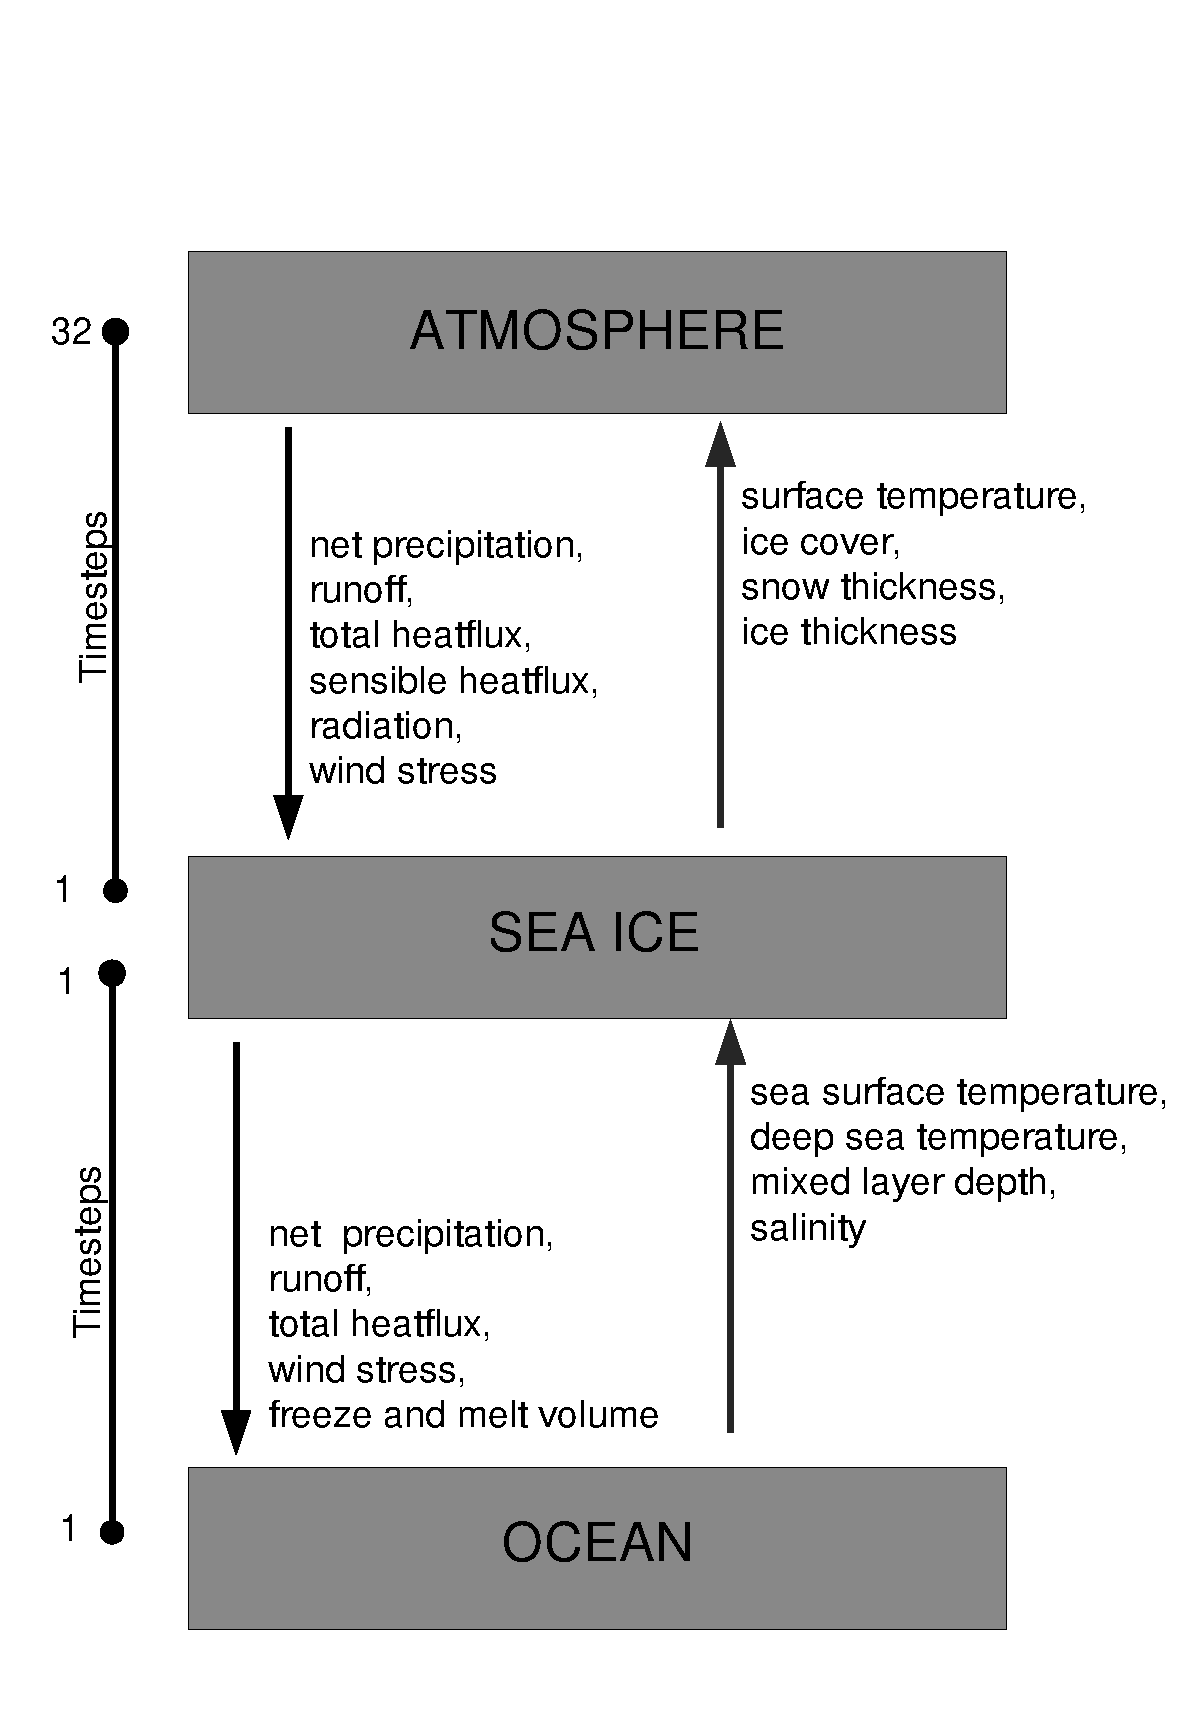
\includegraphics[width={14cm}]{Pics/modules_icemod_couple}
\caption[]{Schematic illustration of the model coupling.}
\label{couplefig}
\end{figure}

\begin{figure}[p]
\vspace{-2cm}
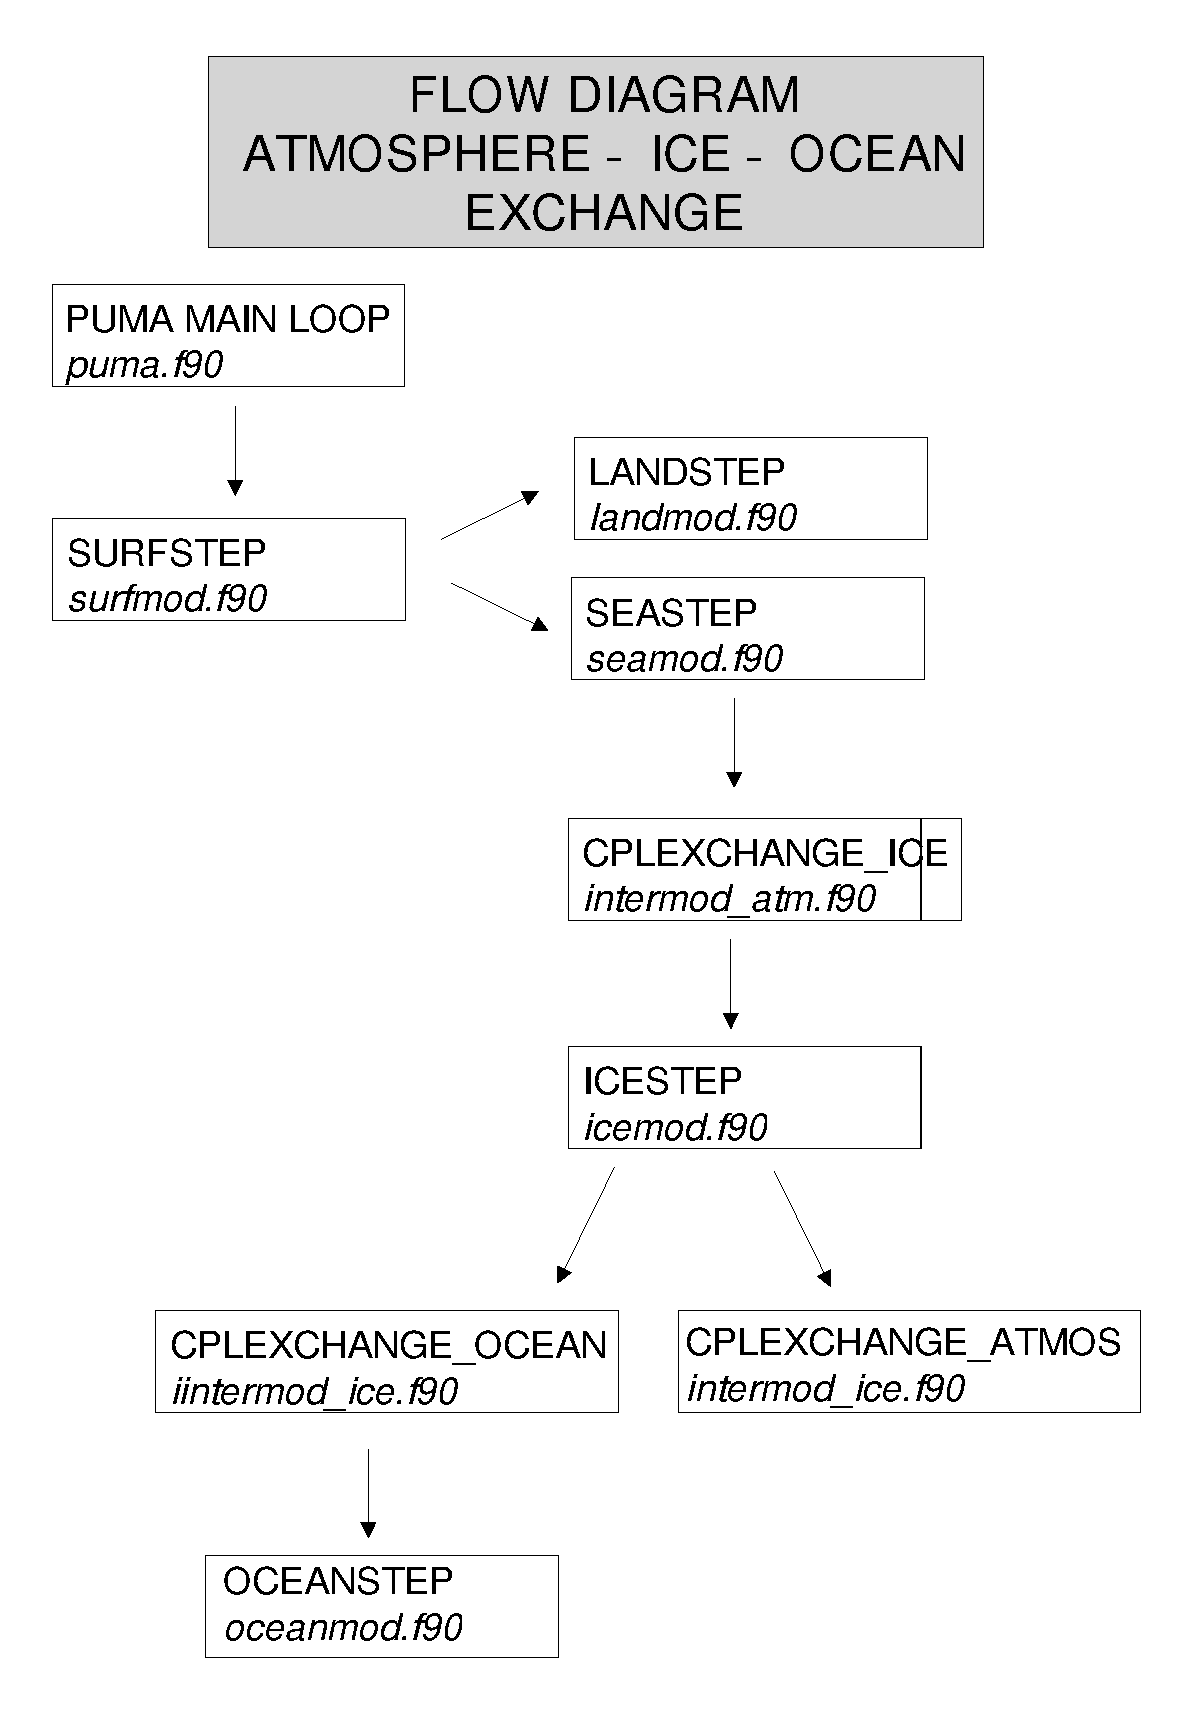
\includegraphics[width={14cm}]{Pics/modules_icemod_pumaflow}
\caption[]{Subroutine flow when no external coupler is used.}
\label{pumaflowfig}
\end{figure}


%----------------------------------------------------------------------------

\clearpage
\begin{center}
\begin{tabular}{|p{14cm}|}
\hline
\vspace{-5mm} \section{icemod.f90} \vspace{-5mm} \\
\hline
\vspace{1mm} {\bf General} The module {\module icemod.f90}
contains subroutines to compute sea ice cover and thickness.
The interface to the main PLASIM module is given by the subroutine
{\sub icestep}, which is called by {\sub cplexchange\verb#_#ice}
(defined in {\module intermod\verb#_#atm.f90}), which is called by
{\sub seastep} (defined in {\module seamod.f90}). \vspace{3mm} \\
\hline
\vspace{1mm} {\bf Input/Output} {\module icemod.f90} requires the file
{\file ice\verb#_#flxcor} if NFLXCORR is set to a negative value.
If NOUTPUT is set to 1, the output files {\file fort.75} containing
global fields of ice model data and the file {\file fort.76}
containing diagnostic ice data are produced (for details,
see the reference manual). Both output files are in service format.
The module is controlled by the namelist {\nam icepar} in the file
{\file ice\verb#_#namelist}. \vspace{1mm} \\
\begin{tabular}{p{3cm} p{2cm} p{6cm} p{2cm}}
Parameter  & Type    & Purpose 					& default \\
NDIAG	   & INTEGER & Diagnostic output every NDIAG time steps	& 160	  \\
NOUT	   & INTEGER & Model data output every NOUT time steps	& 32	  \\
NOUTPUT	   & INTEGER & Icemodel output (0=no,1=yes)		& 1	  \\
NFLXCORR   & INTEGER & Time constant for restoring $(>0)$, no flux correction $(=0)$, use fluxcorrection from file $(<0)$ & $360\,d$ \\
\end{tabular} \vspace{3mm} \\
\hline
\vspace{2mm} {\bf Structure} {\module icemod.f90} uses the module
{\modu icemod} which is not dependent on the module {\modu pumamod}.
Subroutine {\sub iceini} reads the namelist and, when required,
the flux correction from the file {\file ice\verb#_#flxcor}.
Subroutine {\sub icestep} calls {\sub cplexchange\verb#_#atmos}
(defined in {\module intermod\verb#_#ice}) to get the atmospheric
forcing fields. If the {\nam sea\verb#_#namelist} parameter NICE is
set to 1, the subroutine {\sub subice} is called, which calculates
ice cover and thickness. Otherwise, climatological data, interpolated
to the current time step by {\sub iceget} are used. If an ice cover
is present, the surface temperature is calculated in {\sub skintemp}.
Otherwise, the surface temperature is set to the sea surface temperature
calculated by the ocean model. Every NCPL\verb#_#ICE\verb#_#OCEAN
(defined in {\nam sea\verb#_#namelist}) time steps, the external
subroutine {\sub cplexchange\verb#_#ocean} (defined in
{\module intermod\verb#_#ice}) is called to pass the atmospheric
forcing to and retrieve oceanic data from the ocean module
{\module oceanmod.f90}. The oceanic data is used for ice calculations
in the next time step. \vspace{3mm} \\
\hline
\end{tabular}
\end{center} 

%--------------------------------------------------------------------------------

\clearpage
\begin{center}
\begin{tabular}{|p{14cm}|}
\hline
\vspace{-5mm} \section{oceanmod.f90} \vspace{-5mm} \\
\hline
\vspace{1mm} {\bf General} The module {\module oceanmod.f90} contains
a mixed layer ocean model, i.e. subroutines to compute sea surface
temperature and mixed layer depth. The interface to the main PLASIM
module is via the module {\module icemod.f90} given by the subroutine
{\sub oceanstep}, which is called by {\sub cplexchange\verb#_#ocean}
(defined in {\module intermod\verb#_#ice}).  \vspace{3mm} \\
\hline
\vspace{1mm} {\bf Input/Output} {\module oceanmod.f90} requires the file {\file ocean\verb#_#flxcor} if NFLXCORRSST or NFLXCORRMLD is set to a negative value. If NOUTPUT is set to 1, the output file {\file fort.31} containing global fields of ocean model data in service format is produced (for details, see the ice modul section of the reference guide). The module is controlled by the namelist {\nam oceanpar} in the file {\file ocean\verb#_#namelist}. \vspace{1mm} \\
\begin{tabular}{p{3cm} p{2cm} p{6cm} p{2cm}}
Parameter   & Type    & Purpose 			        & default \\
NDIAG	    & INTEGER & Diagnostic output every NDIAG time steps	& 480	  \\
NOUT	    & INTEGER & Model data output every NOUT time steps	& 32	  \\
NOUTPUT	    & INTEGER & Oceanmodel output (0=no,1=yes)		& 1	  \\
NFLXCORRMLD & INTEGER & Time constant for restoring mixed layer depth $(>0)$, no flux correction $(=0)$, use fluxcorrection from file $(<0)$ & $60\,d$ \\
NFLXCORRSST & INTEGER & Time constant for restoring sea surface temperature $(>0)$, no flux correction $(=0)$, use fluxcorrection from file $(<0)$ & $60\,d$ \\
\end{tabular} \vspace{3mm} \\
\hline
\vspace{2mm} {\bf Structure} {\module oceanmod.f90} uses the module
{\modu oceanmod} which is not dependent on the module {\modu pumamod}.
Subroutine {\sub oceanini} reads the namelist and, when required,
the flux corrections from the file {\file ocean\verb#_#flxcor}.
Subroutine {\sub oceanstep} calls {\sub mixocean}, which calculates
mixed layer depth and temperature. If an ice cover is present, mixed
layer depth is set to the climatological value and the sea surface
temperature is set to the freezing temperature. For details of the
mixed layer model, see the Planet Simulator Reference Manual.  \vspace{3mm} \\
\hline
\end{tabular}
\end{center} 

%------------------------------------------------------------------------

